\documentclass[12pt,aspectratio=169]{beamer}
\usepackage[utf8]{inputenc}
\usepackage[T1]{fontenc}
\usepackage{lmodern}
%\usetheme{Malmoe}
\usetheme{Fedora169}
\usepackage{graphicx}
\usepackage{newverbs}

\newverbcommand{\tc}{\color{blue}}{}

%\usebackgroundtemplate{\includegraphics[width=\paperwidth,height=\paperheight]{./images/background.jpg}}

\begin{document}
	\author{Lukáš Růžička (lruzicka@redhat.com)}
	\title{Bugzilla zabije i Godzillu}
	\subtitle{aneb Jak užitečně hlásit bugy}
	\titlegraphic{
\includegraphics[height=2cm]{buggie.png}}
	\institute{Fedora QE}
	\date{}
%	\subject{Fedora 29}
	%\setbeamercovered{transparent}
	\setbeamertemplate{navigation symbols}{}

\begin{frame}[plain]
	\maketitle 
\end{frame}

\section{Úvod}

\begin{frame}{Co je Bugzilla?}
Bugzilla je systém na sledování chyb. Mezi nejdůležitější vlastnosti patří:

\begin{itemize}
\item open source
\item vhodný na sledování chyb
\item velmi konfigurovatelný
\item pamatuje si historii
\item robustní a stabilní
\item bezpečný
\item různá rozhraní (konfigurovatelná a lokalizovatelná)
\end{itemize}

Více na {\color{blue}\url{www.bugzilla.org}}.
\end{frame}

\begin{frame}{Bugzilla ve Fedoře}
Ve Fedoře se pro sledování chyb také používá Bugzilla. Kdokoliv se do ní může přihlásit a podílet se hlášení nebo řešení problémů a chyb. Fedoří Bugzillu hostuje Red Hat a také ji používá.

\begin{itemize}
	\item Red Hat
	\item JBoss
	\item Fedora
	\item komunitní produkty
	\item vnitřní produkty
\end{itemize}

Bugzilla Red Hatu je dostupná na {\color{red}\url{bugzilla.redhat.com}}.
\end{frame}

\section{Hlášení chyb}
\begin{frame}{Proč sledovat chyby?}

\begin{itemize}
	\item nahlášení problému
	\item organizace času, plánování, odhady
	\item spolupráce s ostatními
	\item sdílení nápadů a vědomostí
	\item zobrazení postupu
	\item nalezení řešení
\end{itemize}
\end{frame}

\begin{frame}{Proč byste měli uvažovat o nahlášení chyby?}
Aby se ostatní dozvěděli, že  \ldots{}
\begin{itemize}
	\item jste asi našli chybu
	\item chcete, aby se chyba opravila
	\item máte nějaký zvláštní hardware nebo nastavení
	\item máte nový nápad a přístup
	\item potřebujete zkrátka něco jiného
\end{itemize}

\end{frame}

\begin{frame}{Co by mohla být chyba?}
Chyba by mohlo být všechno, co se nějakým způsobem nechová podle našeho očekávání:
\begin{itemize}
	\item nespouští se to
	\item padá to
	\item běhá to divně
	\item cosi to hlásí
	\item nedělá to, co má dělat\footnote{Když chcete navrhnout nové funkce, kontaktujte upstream.}
	\item a další
\end{itemize}

\end{frame}

\begin{frame}{Než to ohlásím}
Popřemýšlejte o základních věcech, které o problému víte, například \ldots

\begin{itemize}
	\item co se stalo?
	\item kdy? 
	\item jak? 
	\item jak často?
	\item proč (jestli to víte)?
	\item proč se to nemělo stát?
\end{itemize}	
\end{frame}

\begin{frame}{Opakování chyby}
	\begin{enumerate}
		\item Zkuste chybu zopakovat.
		\item Zapište si kroky, které je k tomu potřeba udělat.
		\item Zkuste najít nejkratší postup k chybě, tzv. \textbf{minimal reproducer}.
		\item Zkuste změnit nějaké kroky, jestli se náhodou chyba nevyřeší.
		\item Zkuste totéž v čistém uživatelském profilu.
		\item Zkuste najít způsob, jak se chybě vyhnout (workaround).
	\end{enumerate}
\end{frame}

\begin{frame}{Získávání a poskytování informací}
Chcete-li, aby chybové hlášení bylo dobré, měli byste k němu připojit další informace:
\begin{itemize}
	\item systémové logy a informace
	\item výpisy z dotčené aplikace
	\item screenshoty nebo videa
\end{itemize}
\end{frame}

\section{Sběr informací}
\begin{frame}{ABRT}
\textbf{Automatic Bugzilla Reporting Tool} je služba, která hlídá váš systém a analyzuje problémy.
\begin{itemize}
	\item předinstalován
	\item zaznamenává pády a sbírá data
	\item ulehčuje hlášení chyb
	\item někdy nepomůže
	\item použijte {\color{blue}\texttt{abrt}}, {\color{blue} \texttt{abrt-cli}} na CLI
	\item nebo {\color{blue} \texttt{gnome-abrt}} v GUI 
\end{itemize}
\end{frame}

\begin{frame}[fragile]{Získání logů pomocí \textbf{journalctl}}
\textbf{journalctl} je rozhraní pro přístup k systémovým zprávám. Lze je filtrovat pomocí následujících možností.

\begin{description}
	\item[-\,-\,boot] zprávy od posledního startu
	\item[-\,-\,unit] zprávy od konkrétní služby
	\item[-\,-\,follow] zprávy se zobrazují živě
	\item[-\,-\,since] zprávy od určitého časového bodu
	\item[-\,-\,until] zprávy do určitého časového bodu
\end{description}

\vspace{5pt}

See {\color{blue}\texttt{man journalctl}} for more info.
\end{frame}

\begin{frame}{Získání logů postaru}
\begin{itemize}
	\item adresář {\color{blue} \texttt{/var/log/}} pro některé logy
	\item program {\color{blue} \texttt{dmesg}} k prozkoumání kernelových logů 
	\item spuštění aplikace z terminálu pro zobrazení případných zpráv na {\color{blue}\texttt{stdout}} a {\color{blue}\texttt{stderr}}
	\item adresáře {\color{blue} \texttt{$\sim$/.local}}, {\color{blue} \texttt{$\sim$/.config}}, a {\color{blue} \texttt{/etc}} s nastavením 
	\item zkuste program spustit s přepínačem {\color{blue} \texttt{-v}} pro větší ukecanost
\end{itemize}	
\end{frame}

\begin{frame}{Směrování výstupu}
Aplikace posílají zprávy na \textbf{stdout} a \textbf{stderr}. Někdy se může hodit přesměrovat je do souboru.
\begin{description}
	\item[>] stdout do souboru
	\item[2>] stderr do souboru
	\item[2>\&1] stderr do stdout
	\item[\&>] všechno do souboru
\end{description}

Například:\\ {\color{blue} \texttt{journalctl -b > logs-since-boot.txt}}

\end{frame}

\begin{frame}{Kopírování logů z počítače ven}
Někdy nemůžete kopírovat informace pomocí \textbf{Ctrl-C \& Ctrl-V}, protože to systém neumožňuje (console, virtuálka). Lze však použít jinou metodu:

\begin{itemize}
 \item pomocí \textbf{scp} nebo \textbf{rsync}
 \item pomocí \textbf{fpaste} nebo \textbf{dpaste}	
\end{itemize}
\end{frame}

\begin{frame}{Použití rsync nebo scp}
\begin{itemize}
	\item {\color{blue} \texttt{scp file.txt username@<r-system>:/remote/directory/newfile.txt}}
	\item {\color{blue} \texttt{scp username@<r-system>:/remote/file.txt /local/directory/newfile.txt}}
	\item \textbf{rsync} se chová podobně
	\item Více v manuálových stránkách.
\end{itemize}
\end{frame}

\begin{frame}{Pomocí dpaste}
Ve Fedoře se standardně nabízí \textbf{fpaste}, ale vrací ukrutně dlouhý hash -- \texttt{Kut1tUlXWJvpwI2QEcX5EA}. 

\vspace{5pt}

\textbf{dpaste} vrací pouze 4 znaky, což se daleko lépe pamatuje -- \texttt{vWVF}.

\vspace{5pt}

\textbf{dpaste} je k dispozici z {\color{blue}\url{https://github.com/lruzicka/dpaste.git}}.

\vspace{5pt}

A zkopírované snippety lze přečíst z {\color{blue}\url{http://dpaste.de}}.

\end{frame}

\section{Používáme Bugzillu}
\begin{frame}{Nově v Bugzille}
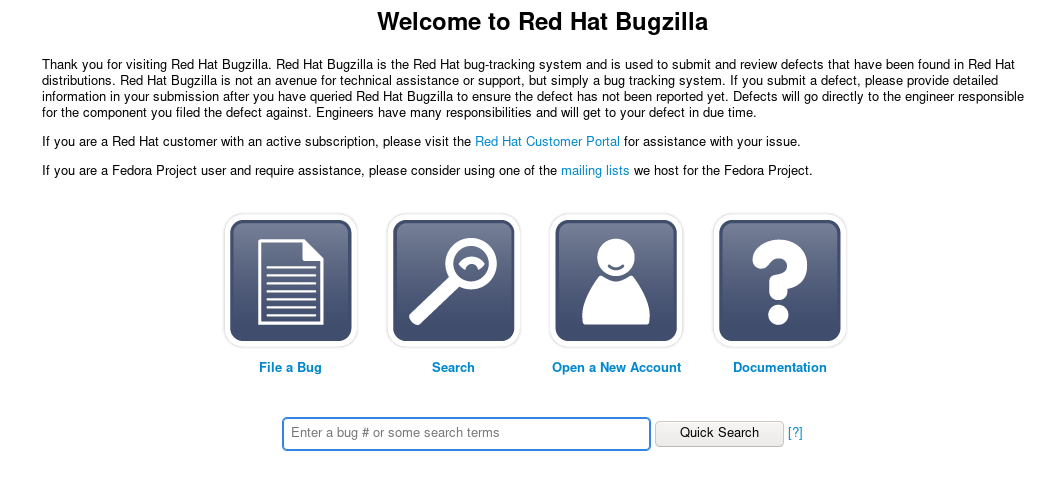
\includegraphics[width=10cm]{images/bz_new.png}
\end{frame}

\begin{frame}{Přihlášení do Bugzilly}
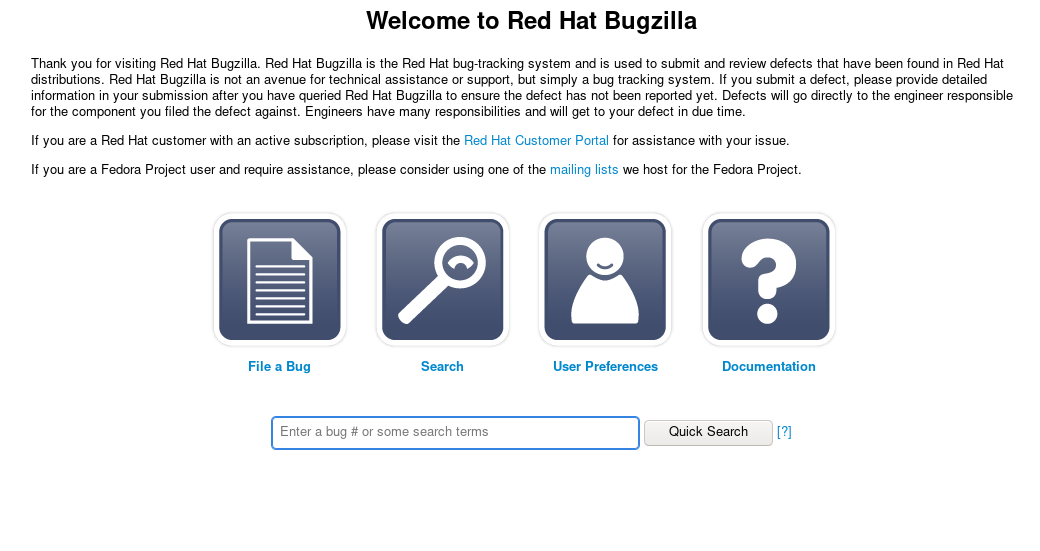
\includegraphics[width=10cm]{images/bz_logged.png}
\end{frame}

\begin{frame}{Klasifikace chyby}
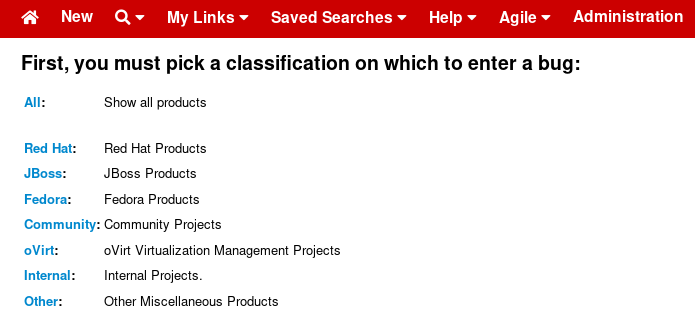
\includegraphics[width=10cm]{images/bz_classification.png}
\end{frame}

\begin{frame}{Výběr správného produktu}
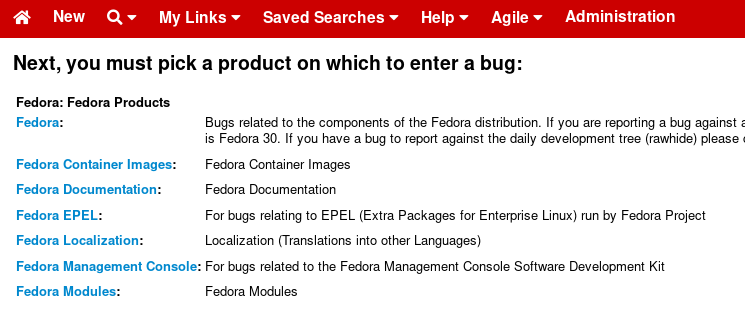
\includegraphics[width=10cm]{images/bz_product.png}
\end{frame}

\begin{frame}{Hlášení chyby (část 1)}
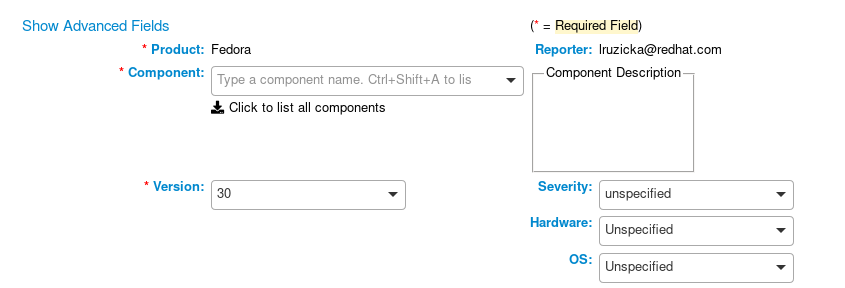
\includegraphics[width=10cm]{images/bz_header.png}
\end{frame}

\begin{frame}{Hlášení chyby (část 2)}
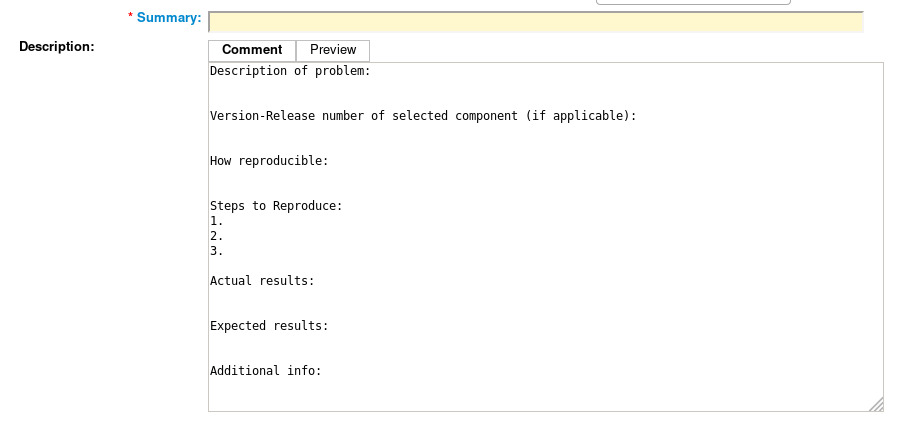
\includegraphics[width=10cm]{images/bz_description.png}
\end{frame}

\begin{frame}{Popis chyby}
\begin{itemize}
	\item Co je ze problém?
	\item Kdy se objevuje?
	\item Jak to ovlivňuje práci?
	\item Proč je to problém?
	\item další
\end{itemize}
\end{frame}

\begin{frame}[fragile]{Verze komponenty}
Napište verzi problematické komponenty a také verze dalších komponent, které mohou hrát roli.
\begin{itemize}
	\item {\color{blue}\textbf{About}} menu v GUI
	\item {\color{blue}\texttt{-v}} nebo {\color{blue}{\verb|--version|}} volba na CLI (nebo \texttt{man})
	\item {\color{blue}\texttt{rpm -q}} pro verze instalovaných balíčků
	\item {\color{blue}\texttt{dnf info}} pro instalované a dostupné balíčky
\end{itemize}
\end{frame}

\begin{frame}{Jak reprodukovatelné}
\begin{itemize}
	\item Always
	\item Sometimes -- kdy přesně?
	\item Za určitých podmínek -- popište je
	\item Heisenbug 
\end{itemize}
\end{frame}

\begin{frame}{Kroky vedoucí k chybě}
Co musím udělat, aby se chyba projevila?
\begin{itemize}
	\item Jedna činnost v jednom kroku.
	\item Nepřeskakujte kroky, byť se zdají být zjevné.
	\item Pozor na detaily.
	\item Buďte přesní.
\end{itemize}
Ostatní ten bug chtějí taky vidět.
\end{frame}

\begin{frame}{Výsledek}
\begin{description}
	\item[Actual] -- co to dělá?
	\item[Expected] -- co si myslíte, že by to mělo dělat?
\end{description}
\end{frame}

\begin{frame}{Hlášení chyby (část 3)}

\includegraphics[width=10cm]{images/bz_footer.png}
\end{frame}

\begin{frame}{Nemáte ani páru, co se děje?}

{\Large Nahlašte to i tak!}
\end{frame}

\section{Otázky}

\begin{frame}{Q\&A}

{\Large Znáte to, o té líné hubě?}
\end{frame}

\end{document}